\documentclass[10pt,a4paper]{article}
\usepackage[utf8]{inputenc}
\usepackage{amsmath,amssymb}
\usepackage{enumitem}
\usepackage{float}
\usepackage{graphicx}
\usepackage{geometry}
% Configuración de márgenes
\geometry{
    top=2.4cm,      % margen superior
    bottom=1.25cm, % margen inferior
    left=2.25cm,     % margen izquierdo
    right=1.25cm     % margen derecho
}
\begin{document}
\section*{Problema 1}
La ecuación del movimiento armónico simple (MAS) de un péndulo simple se deriva utilizando supuestos que la hacen válida para pequeños desplazamientos. Durante un experimento, se suspende una bola esférica con un hilo de 1,20 m de longitud y se desplaza el péndulo 28°. Calcule el período del péndulo suponiendo un pequeño desplazamiento y utilizando la ecuación:

\[
T = 2\pi \sqrt{\frac{L}{g}} \times \left(1 + \frac{1^2}{2^2}\sin^2\frac{\theta}{2} + \frac{1^2 \cdot 3^2}{2^2 \cdot 4^2}\sin^4\frac{\theta}{2}\right)
\]

(i) Indique el valor más preciso, (ii) Determine el error porcentual del otro valor comparándolo con el valor que usted considera preciso.
\vspace{8cm}
\section*{Problema 2}
El movimiento de un péndulo simple se aproxima al movimiento armónico simple (MAS) para pequeños desplazamientos. Supongamos que desplazamos una esfera suspendida de un hilo de 1,4 m de longitud 25,0°. (i) ¿Cuál es su período suponiendo un pequeño desplazamiento? (ii) ¿Cuál es el período utilizando los tres términos de la ecuación dada:

\[
T = 2\pi \sqrt{\frac{L}{g}} \times \left(1 + \frac{1^2}{2^2}\sin^2\frac{\theta}{2} + \frac{1^2 \cdot 3^2}{2^2 \cdot 4^2}\sin^4\frac{\theta}{2}\right)
\]
\vspace{8cm}
\vspace{8cm}
\section*{Problema 3}
Un reloj de pie con un péndulo de 1,00 m de longitud cuelga de una torre. La masa del péndulo es de 0,500 kg. Un conductor, por desgracia, choca contra la torre, haciéndola vibrar. Si el péndulo estaba inicialmente en reposo en su posición de equilibrio, ¿Cuántos ciclos por segundo dará?
\vspace{6cm}
\section*{Problema 4}
Una plomada desplazada un pequeño ángulo de su posición de equilibrio tiene un período de 1,23 s en la Tierra. ¿Cuál es el período de este péndulo simple cuando se lleva a la superficie del planeta K, donde $g$ es $13,2 \text{ m/s}^2$?
\vspace{6cm}
\section*{Problema 5}
Construyes un péndulo simple de 0,84 m de longitud con una cuerda ligera y lo desplazas 4,30° en un lado antes de soltarlo para que oscile. A continuación, duplicas el ángulo de desplazamiento a 8,60° en el mismo lado. ¿Cuál es la diferencia entre los periodos de tiempo para los dos ángulos utilizados?
\vspace{6cm}
\section*{Problema 6}
Un péndulo simple tiene una longitud de 1,35 m. El péndulo se desplaza 5,60° hacia un lado y se deja oscilar. Determina el tiempo transcurrido desde su lanzamiento hasta que su aceleración es cero.
\vspace{6cm}
\section*{Problema 7}
Un péndulo decorativo en un reloj de pared está hecho de una masa esférica de 250 gramos recubierta de oro que cuelga de un cordón de 35 cm de largo. El propietario pone en marcha el péndulo a las 4:00 p. m. desplazándolo 3,0 cm hacia un lado. El péndulo es casi perfecto, con una constante de amortiguación de $2,5 \times 10^{-5} \text{ kg/s}$. Calcule la amplitud y el número de ciclos que realiza el péndulo a las 11:00 p. m.
\vspace{6cm}
\section*{Problema 8}
Una masa de 125 g cuelga de un hilo sin masa de 105 cm de longitud. La masa comienza a desplazarse 8 grados. Calcula cuántas veces pasa la masa por la posición de equilibrio en 10,0 s.
\vspace{6cm}
\section*{Problema 9}
Una masa suspendida de una cuerda de 1,2 m de longitud oscila como un péndulo. La velocidad del péndulo en el punto de equilibrio es de 1,50 m/s. Calcula el ángulo de desplazamiento ($\theta_{\text{máx}}$) de la masa en grados.
\vspace{6cm}
\section*{Problema 10}
Un vehículo espacial autónomo mueve un péndulo entre dos planetas. En Júpiter, el péndulo tiene un período de 1,2 s ($g = 24,8 \text{ m/s}^2$). El péndulo se traslada a otro planeta donde su período es de 3,2 s. Calcula la aceleración gravitatoria en dicho planeta.
\vspace{6cm}
\section*{Problema 11}
Una barra de madera regular de L metros de longitud, masa M y composición uniforme, pivota mediante un clavo en un punto (0,3L) medido desde un extremo de la barra. Para la barra oscilando en ángulos pequeños, derive una expresión para la frecuencia $f$ de la oscilación.
\vspace{6cm}
\section*{Problema 12}
Un adorno consiste en una barra de 22 cm de largo y 270 g de masa. Un extremo sirve de pivote, mientras que el extremo opuesto lleva una masa esférica, que puede considerarse una masa puntual, de 48 g. Si la combinación barra-masa oscila como un péndulo, calcule el periodo de su movimiento.
\vspace{6cm}
\section*{Problema 13}
Un trozo de madera regular de longitud L pivota alrededor de una posición x medida desde su centro de masa. Calcula el valor de x que produce el menor período de oscilación. Expresa x en función de L.
\vspace{6cm}
\section*{Problema 14}
El momento de inercia es fundamental en el diseño de objetos y sistemas que experimentan rotaciones. En un modelo de grúa, una barra de 12 kg mide 1,3 m de longitud. Su centro de masa se encuentra a 25 cm del eje de rotación. La barra oscila alrededor del eje de rotación como un péndulo con una frecuencia de 0,55 Hz. Calcule el momento de inercia de la barra respecto al eje de rotación.
\vspace{6cm}
\section*{Problema 15}
Imagina una esfera llamada "OrbMover" suspendida del techo, inicialmente con un ángulo de reposo de 9,5° respecto a la vertical. Determina el nuevo ángulo que debe alcanzar OrbMover para duplicar su energía potencial y cinética totales.
\vspace{6cm}
\section*{Problema 16}
Un péndulo conocido como "TimeSwing" comienza su movimiento desde un estado estacionario con una desviación de 10° respecto al eje vertical. Oscila de un lado a otro con una frecuencia regular de 2,8 Hz. Sin considerar ninguna resistencia, determine la posición angular en radianes del péndulo TimeSwing en $t = 0,28 \text{ s}$.
\vspace{6cm}
\section*{Problema 17}
Un péndulo llamado "SwingMotion" oscila con un desplazamiento angular máximo de 12,0° respecto a la posición de equilibrio. ¿Qué fracción de su periodo transcurre entre +6,0° y -6,0°? Suponga que el movimiento sigue principios armónicos simples.
\vspace{6cm}
\section*{Problema 18}
"GraviSwing" es un péndulo simple que oscila con una frecuencia inicial $f$. Determina la nueva frecuencia de oscilación de GraviSwing cuando experimenta una aceleración hacia arriba de $0,6g$.
\vspace{6cm}
\section*{Problema 19}
Imagina una esfera de 296 g de masa unida a una cuerda de 0,64 m de longitud que cuelga del techo. La esfera se suelta con un ángulo de 14° respecto a la vertical. Suponiendo que el movimiento es armónico simple, calcula la frecuencia de oscilación de la esfera.
\vspace{6cm}
\section*{Problema 20}
Imagina una bola que actúa como un péndulo, suspendida del techo de un armario mediante una cuerda de 52 cm de longitud. Calcula el periodo de oscilación de la bola cuando el armario cae en caída libre.
\vspace{6cm}
\section*{Problema 21}
Imagina una bola de metal suspendida por una cuerda, que oscila de un lado a otro con una frecuencia determinada ($f$). Ahora bien, si colocáramos todo este conjunto en un ascensor que desciende con una aceleración de $0,28g$, ¿Cuál sería la nueva frecuencia ($f'$) de las oscilaciones de la bola?
\vspace{5cm}
\section*{Problema 22}
En un mecanismo de reloj, una rueda de péndulo de 0,96 cm de radio, unida a un resorte helicoidal, vibra a 3,20 Hz. Si un par de torsión de $2,1 \times 10^{-5} \text{ Nm}$ produce una rotación de 60°, ¿Cuál es la masa de la rueda?
\begin{figure}[H]
    \begin{flushleft}
        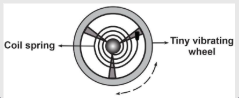
\includegraphics[width=0.4\textwidth]{figure/grafica1.png}
        \label{fig:pendulum}
    \end{flushleft}
\end{figure}
\vspace{2cm}
\section*{Problema 23}
Un disco acrílico de 2,30 kg con un radio de 30,0 cm está suspendido por un gancho metálico a través de un orificio situado a 5,00 cm de su borde, lo que le permite oscilar como un péndulo. ¿Cuál es el periodo de sus pequeñas oscilaciones?
\begin{figure}[H]
    \begin{flushleft}
        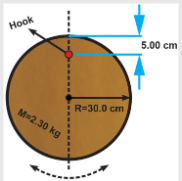
\includegraphics[width=0.4\textwidth]{figure/grafica2.png}
        \label{fig:pendulum2}
    \end{flushleft}
\end{figure}
\vspace{4cm}
\section*{Problema 24}
Un inventor crea un dispositivo que consiste en un altavoz suspendido del techo mediante una cuerda. Al comenzar a oscilar, el altavoz reproduce un ritmo de batería cada vez que alcanza la máxima distancia desde su posición de equilibrio. Dado que el altavoz emite 120 pulsaciones por minuto (ppm) al comenzar a oscilar, ¿Cuál es la longitud de la cuerda?
\vspace{8cm}
\section*{Problema 25}
Un estudiante coloca una regla en el borde de una mesa. Sujeta un extremo de la regla dentro de la mesa y deja el otro extremo fuera. Luego, golpea el extremo que sobresale de la mesa a una velocidad de 32 km/h. Esto provoca que la regla oscile en movimiento armónico simple (MAS). Dado que la parte de la regla que sobresale de la mesa mide 15 cm, el período de oscilación es de 0,78 s y la amplitud es de 7 cm, determine la velocidad y la aceleración máximas del extremo oscilante de la regla. Exprese la aceleración máxima como un porcentaje de la aceleración gravitatoria $g$.
\vspace{10cm}
\section*{Problema 26}
Un profesor de física está de gira impartiendo conferencias en varios lugares. Para ello, lleva consigo un péndulo. Desea que el péndulo tenga un periodo exacto de 1,000 s. En Florida, el profesor mide el valor de '$g$' en $9,798 \text{ m/s}^2$ y en Anchorage en $9,819 \text{ m/s}^2$. Por otro lado, el valor de '$g$' en Marte es de $3,721 \text{ m/s}^2$. Determina la longitud del péndulo del profesor en Florida y el ajuste de longitud que realiza al pasar de Florida a Anchorage. Además, calcula la longitud del péndulo en Marte para que el periodo sea el mismo.
\vspace{8cm}
\section*{Problema 27}
Un reloj de pie tradicional utiliza un péndulo compuesto para medir el tiempo, el cual consta de dos varillas metálicas interconectadas que oscilan alrededor de un punto de pivote superior fijo. Suponga que ambas varillas tienen la misma longitud, 0,75 metros cada una. La varilla superior tiene una masa de 1,5 kg y la inferior, de 1,0 kg. Calcule el período de oscilación de este sistema de péndulo.
\vspace{8cm}
\section*{Problema 28}
Una exhibición de museo presenta un gran péndulo decorativo que oscila de un lado a otro. El péndulo consiste en una pesada masa $m$ en el extremo de una varilla larga y ligera de longitud $l$. Teniendo en cuenta la aceleración gravitatoria $g$, derive la ecuación para el desplazamiento angular $\theta(t)$ del péndulo, dado que el desplazamiento angular máximo es pequeño. Suponga que el péndulo experimenta un movimiento armónico simple para pequeños desplazamientos. Utilice la relación $\tau = I\alpha$.
\begin{figure}[H]
    \begin{flushleft}
        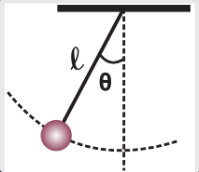
\includegraphics[width=0.4\textwidth]{figure/grafica3.png}
        \label{fig:pendulum3}
    \end{flushleft}
\end{figure}
\vspace{6cm}
\section*{Problema 29}
Una placa metálica en forma de horquilla oscila entre los polos norte y sur de un imán. Su amplitud se reduce al 42,8 \% de la amplitud inicial en 8,60 s. Calcula la constante de tiempo.
\vspace{10cm}
\section*{Problema 30}
La fuerza gravitatoria puede utilizarse como fuerza restauradora para una masa $m_0$ que oscila en un hueco perforado a través del centro de una masa esférica (un diámetro). Para una esfera de masa $M_s$ y radio $R_s$, se demuestra que una masa oscilante con posición $x$, donde $r \le x \le R_s$, experimenta una fuerza gravitatoria neta de la masa esférica encerrada por $r$, donde $r \le x$, mientras que la masa de la capa esférica en $x > r$ no contribuye a la fuerza gravitatoria neta de la masa oscilante. Para una esfera con densidad uniforme, derive una expresión para la fuerza gravitatoria sobre la masa oscilante. Exprese el resultado utilizando $M_s$, $R_s$, $x$, $m_0$ y cualquier constante deseada.

\end{document}
